\documentclass[11pt,addpoints,answers]{exam}

\usepackage[top=0.5in, left=0.75in, right=0.75in, bottom=.5in]{geometry}
\usepackage{amsmath,amsfonts,nicefrac, amssymb,amsxtra}
\usepackage{mathtools}
\usepackage{multicol}
\usepackage{pdfpages}
\usepackage{setspace}
\usepackage{enumitem}

%\usepackage{mathexam}
%\usepackage{latexsym}
%\usepackage[square, comma, sort&compress, numbers]{natbib}
%\usepackage{moresize}
%\usepackage{algpseudocode}
\usepackage{stmaryrd}
%\usepackage{enumitem}
%\renewcommand{\theenumi}{\alph{enumi}}
\usepackage{tabularx,ragged2e,booktabs,caption}
\usepackage{epstopdf}
\usepackage{epsfig}
\usepackage{setspace}
\usepackage{tikz,pgfplots}
\usetikzlibrary{arrows.meta}
\usetikzlibrary{arrows,decorations.markings}
\pgfplotsset{compat=1.14}
\usepgfplotslibrary{units}
\pgfplotsset{soldot/.style={color=black,only marks,mark=*}}
\pgfplotsset{holdot/.style={color=black,fill=white,only marks,mark=*}}
\usepackage{polynom}
\usepackage{enumerate}
\usepackage{graphicx,wrapfig,lipsum}
\allowdisplaybreaks


\usepackage[utf8]{inputenc}
\usetikzlibrary{decorations}
\usetikzlibrary{decorations.pathreplacing}
%\usepackage{fancyhdr}
\usepackage{array}
\usepackage{parskip}

\renewcommand{\arraystretch}{1.2}
\renewcommand\partlabel{(\thequestion.\arabic{partno})}

\newcommand{\emptybox}[2][\textwidth]{%
  \begingroup
  \setlength{\fboxsep}{-\fboxrule}%
  \noindent\framebox[#1]{\rule{0pt}{#2}}%
  \endgroup
}

\pgfplotsset{compat=1.14}


\begin{document}
\noindent {\Large Quiz, Fall Week 8 \hfill Name: \underline{\hspace{7cm}}}

\noindent {\normalsize {Points possible: \numpoints      \hfill Math 1050-90, Fall 2021, Due 10/26 at 11:59 p.m.}}

{\small \noindent \textbf{Rules/Suggestions:} Write with a dark pencil, so that your work is visible.  \textbf{You are graded on your work, not just answers. Even if you do calculations in your head or on scratch, show work if space is provided. } Write the final answer in the box.

Notes: You are on your honor for this to be your own work.  (You can ask for help on quiz material, but you should not ask for help on specific problems.) }
\begin{questions}


\setlength\columnsep{2cm}

\begin{multicols}{2}
\question[10] Use the change of base property to convert the given expression to an expression with base $e$.
\[\log_3 (36)\]
\vspace*{1.5in}
\begin{flushright}\fbox{%
\begin{minipage}{3 in}
Answer:\\[3ex]
\end{minipage}}\end{flushright}
\columnbreak

\question[10] Solve EXACTLY.  Write the answer in fractions or integers, and your answer may contain one or more logs or natural logs.
\[4^{5x} = 12\]
\vspace*{1.5in}
\begin{flushright}\fbox{%
\begin{minipage}{3 in}
$x=$\\[3ex]
\end{minipage}}\end{flushright}
\end{multicols}

\begin{multicols}{2}
\question[10] Solve EXACTLY.  Check that your answer is not extraneous before entering it.
\[\log_4 (x-1) + \log_4 (x-13) = 3\]
\vspace*{2in}
\begin{flushright}\fbox{%
\begin{minipage}{3 in}
$x=$\\[3ex]
\end{minipage}}\end{flushright}
\columnbreak

\question[10] Expand the logarithm after factoring.
\[\log_5 (x^2 - 36)\]
\vspace*{2in}
\begin{flushright}\fbox{%
\begin{minipage}{3 in}
Answer:\\[3ex]
\end{minipage}}\end{flushright}
\end{multicols}

 \vfill
\pagestyle{empty}
\hspace*{1in}{\Huge \textbf{Page 1}}
\newpage


\begin{multicols}{2}
\question[10] Condense the expression so it contains a single log.
\[\ln(6x) + 5\ln(y) - 2\ln(z)\]
\vspace*{2in}
\begin{flushright}\fbox{%
\begin{minipage}{3 in}
Answer:\\[3ex]
\end{minipage}}\end{flushright}
\columnbreak

\question[10] If $\ln(a) = 7, \ln(b) = 9,$ and $\ln(c)=8$, evaluate the following expression:
\[\ln \bigg(\dfrac{a^2}{b^3 c^4}\bigg)\]
\vspace*{2in}
\begin{flushright}\fbox{%
\begin{minipage}{3 in}
Answer:\\[3ex]
\end{minipage}}\end{flushright}
\end{multicols}

\question Solve the equations.  Write EXACT solutions.  (You should not use a calculator... if you are, you are likely not finding EXACT solutions.)
\begin{multicols}{2}
\begin{parts}

\part[5] $e^{2x}-e^{x} = 6$
\vspace*{3in}
\begin{flushright}\fbox{%
\begin{minipage}{2.75 in}
$x=$\\[3ex]
\end{minipage}}\end{flushright}

\part[5] $5^{x+3} = 5^{4x-12}$
\vspace*{3in}
\begin{flushright}\fbox{%
\begin{minipage}{2.75 in}
$x=$\\[3ex]
\end{minipage}}\end{flushright}
\end{parts}\end{multicols}


 \vfill
\pagestyle{empty}
\hspace*{3in}{\Huge \textbf{Page 2}}


\newpage
\question Find the requested information for the function, writing ``none'' if appropriate. Write asymptotes as equations and intercepts as ordered pairs.
$$ f(x)= 3^{x-2}+1\\$$
\begin{multicols}{2}

\begin{parts}
\part[6] \hspace{1in}\\

\vspace*{-.3in}
\begin{flushright}
\fbox{%
\begin{minipage}{2.5 in}Domain:\\[3ex]
\end{minipage}}
\fbox{%
\begin{minipage}{2.5 in}

Range:\\[3ex]
\end{minipage}}
\end{flushright}


\part[6]

\hspace{1in}\\
\vspace*{.5in}
\begin{flushright}
\fbox{%
\begin{minipage}{2.5 in}

$x$-intercept:\\[3ex]
\end{minipage}}
\fbox{%
\begin{minipage}{2.5 in}

$y$-intercept:\\[3ex]
\end{minipage}}\end{flushright}

 \columnbreak

\part[6] (Hint: it may be easier to find end behavior AFTER you have graphed.)\hspace{1in}\\

\begin{flushright}\fbox{%
\begin{minipage}{2.5 in}
Asymptote:\\[3ex]
\end{minipage}}
\fbox{%
\begin{minipage}{2.5 in}

End behavior:\\
 As $x\rightarrow-\infty$, $f(x)\rightarrow$ \hrulefill\\

   As $x\rightarrow \infty$, $f(x)\rightarrow$ \hrulefill\\
\end{minipage}}
\end{flushright}


\vspace{.5cm}
\part[12] Sketch the
graph, carefully marking intercept(s), the asymptote, and one point with INTEGER coordinates that the function goes through.\\

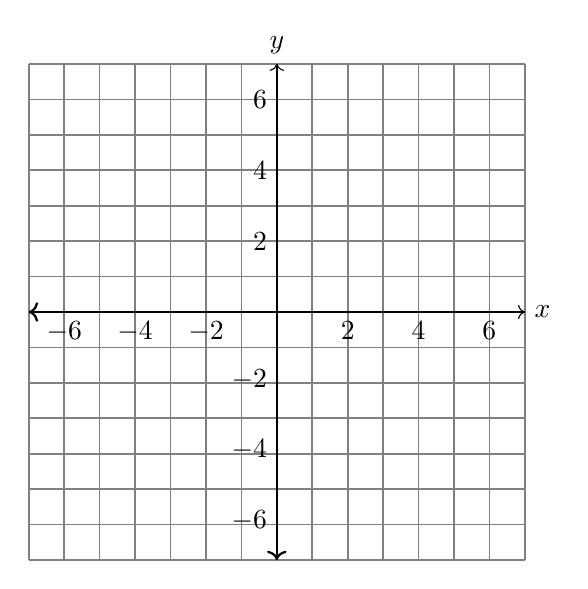
\begin{tikzpicture}[scale=.45]
\draw[help lines][semithick] (-7,-7) grid (7,7);
\draw[<-] [thick] (-7,0) -- (7,0) ;
\draw[<-] [thick] (0,-7) -- (0,7) ;
\foreach \x in {  -6, -4,  -2,  2,  4, 6 } \node[below] at (\x, 0) {$\x$};
\draw[->] (0, 0) -- (7, 0) node[right] {$x$};	% x-axis
\draw[->] (0, -7) -- (0, 7) node[above] {$y$};	% y-axis
\foreach \y/\ytext in { -5.9/-6, -3.9/-4, -1.9/-2,  2/2,4/4, 6/6} \node[left] at (0, \y) {$\ytext$};
\end{tikzpicture}
\end{parts}
\end{multicols}

\end{questions}

  \vfill
\pagestyle{empty}
\hspace*{5in}{\Huge \textbf{Page 3}}



\end{document}
